\documentclass[12pt,oneside]{amsart}
\usepackage{geometry}                % See geometry.pdf to learn the layout options. There are lots.
\geometry{letterpaper}                   % ... or a4paper or a5paper or ... 
%\geometry{landscape}                % Activate for for rotated page geometry
\usepackage[parfill]{parskip}    % Activate to begin paragraphs with an empty line rather than an indent
\usepackage{graphicx}
\usepackage{amssymb}
\usepackage{epstopdf}
\DeclareGraphicsRule{.tif}{png}{.png}{`convert #1 `dirname #1`/`basename #1 .tif`.png}

\title{Kalman Filter Notes}
\author{Aviv Bachan}
%\date{}                                           % Activate to display a given date or no date

\begin{document}
\maketitle
%\section{}
%\subsection{}

%\section{Introduction}
%TBD

\section{Kalman filtering of a simple linear system}
Before going into much detail about the filter itself let's see what it does. Let's start with a simple dynamical system which, for instance, may be taken as representing the position and velocity of a mass on a spring:
\begin{equation}\label{eq:sys}
\begin{aligned}
\dot y_1 &= -2\,y_1 + 2\,y_2 + 1\\
\dot y_2 &= -4\,y_1 + 2\,y_2
\end{aligned}
\end{equation}





The analytical solution for the system of equations is:
\begin{equation}\label{eq:an_sol}
\begin{aligned}
%y_1 &= \frac{3\,\sin{2\,t} + 3\,\cos{2\,t} -1}{2}
y_1 &= 1.5\,\sin{2\,t} + 1.5\,\cos{2\,t} - 0.5
\\
y_2 &= 3\,\cos{2\,t} - 1
\end{aligned}
\end{equation}

\begin{figure}[htbp]
\begin{center}
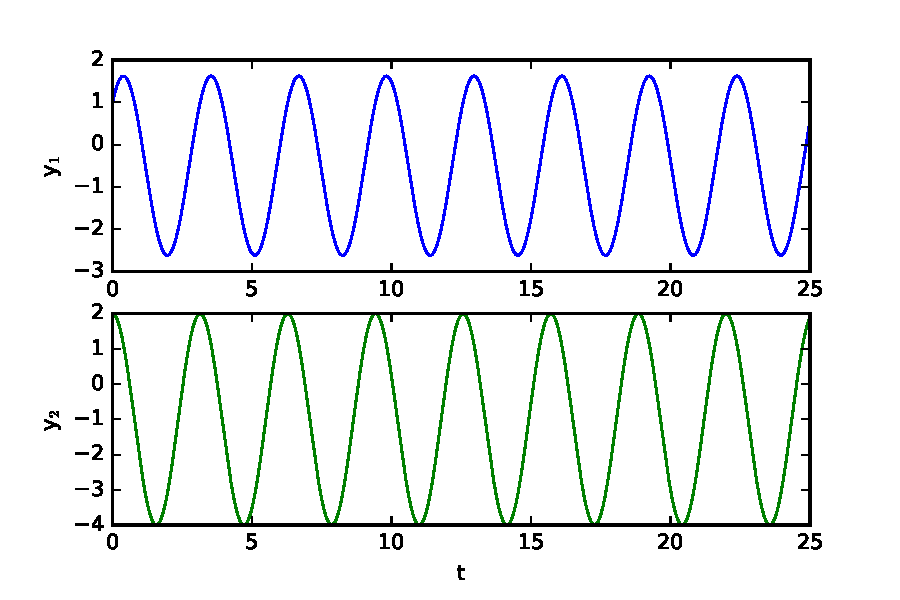
\includegraphics[width = 0.5\textwidth]{Figures/analytical_solution}
\caption{Plot of analytical solution (Equation \ref{eq:an_sol}) for simple dynamical system (Equation \ref{eq:sys}).}
\label{fig:an_sol}
\end{center}
\end{figure}

Let us further assume that our model of the system is imperfect. There are non-linearities in the spring, there is air resistance, wind, and a myriad of other un-accounted for effects. If these effects are uncorrelated then their sum total will have a Gaussian distribution. We can represent this uncertainty by adding noise to our initial value and then at every simulation step to the dynamical system (Figure \ref{fig:stoch_sys}). Note that now the model does not belong anymore to the familiar deterministic models we are used to working with, but rather is now stochastic. Each time the model is simulated (each realization) the result will be different, and this randomness is an inherent characteristic of the \emph{model}, so that no amount of numerical improvement (reduction in step size, etc.) can result in a more accurate output. For non-linear systems the realizations may be wildly different from each other. Nonetheless, for linear systems, the statistical properties of the stochastic system are guaranteed to converge to those of the analytical solution, e.g.\ the mean of the ensemble at any time converges to the true mean. 


\begin{figure}[htbp]
\begin{center}
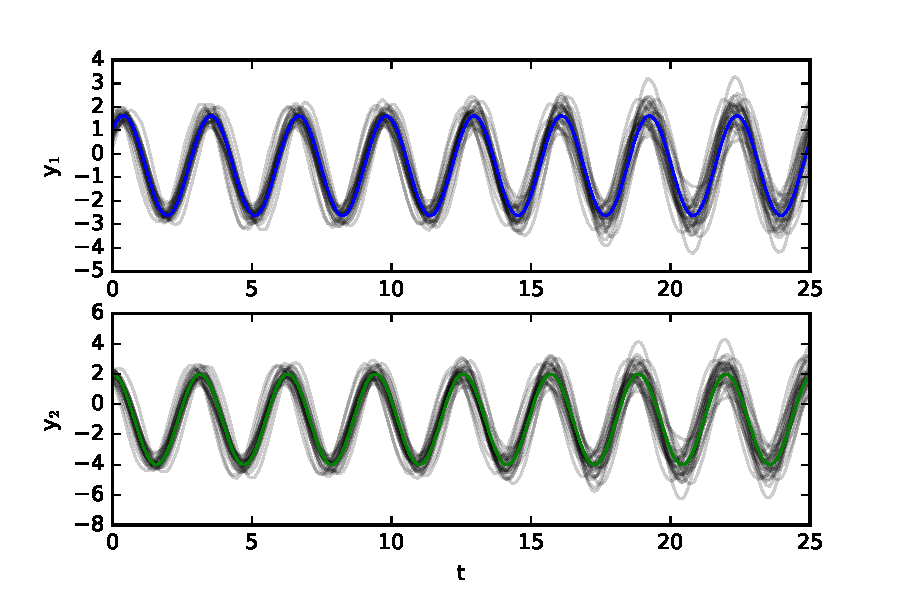
\includegraphics[width = 0.5\textwidth]{Figures/stoch_system}
\caption{Plot of dynamical system with normally distributed noise added to it (gray lines). Blue and green lines are  analytical solution.}
\label{fig:stoch_sys}
\end{center}
\end{figure}

A second source of uncertainty may come from our observations which may themselves be imprecise. For instance, as geochemists are well aware, repeated weighing of a small amount of material will inevitably result in slightly different values, though the amount of material being weighed remains constant. If the sources of error are uncorrelated then this uncertainty too can be represented by a noise term with a Gaussian distribution, which may be different from the uncertainty related to the model (Figure \ref{lab:sensor_noise}). %This distinction between inherent uncertainty (system noise) and observational uncertainty (sensor noise) is an important one.

\begin{figure}[htbp]
\begin{center}
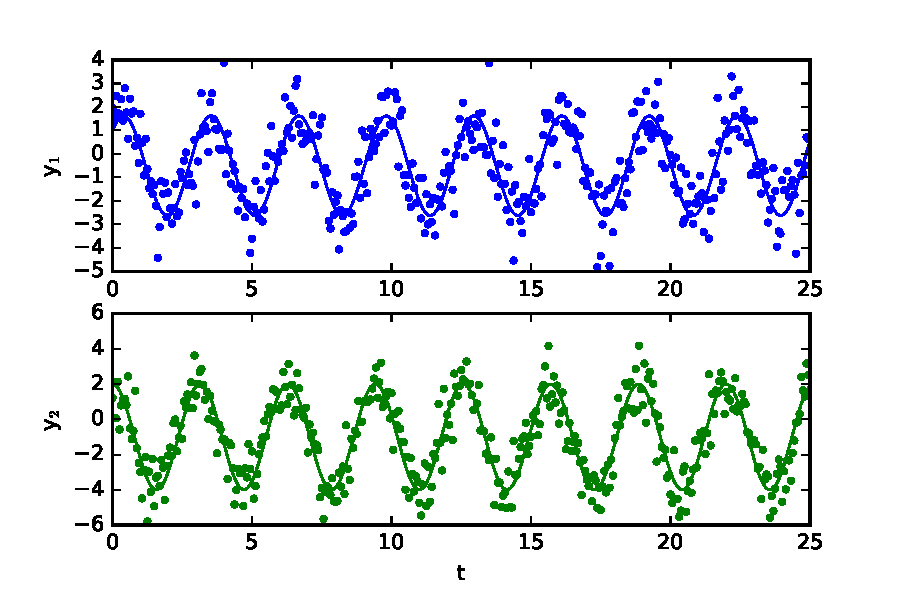
\includegraphics[width = 0.5\textwidth]{Figures/data}
\caption{Analytical solution plus sensor noise.}
\label{lab:sensor_noise}
\end{center}
\end{figure}

The question is then, given these uncertainties can one recover a precise estimate of the states of the system? The Kalman filter does precisely that, and, for linear systems and Gaussian noise, is guaranteed to provide an estimate that is as close as possible to the true (analytical) solution, and is \emph{better than either model or observations alone}. 
%
In Figure \ref{fig:RTS_stoch_data} the output of the Kalman Filter is plotted alongside the noisy model and noisy data. 


\begin{figure}[htbp]
\begin{center}
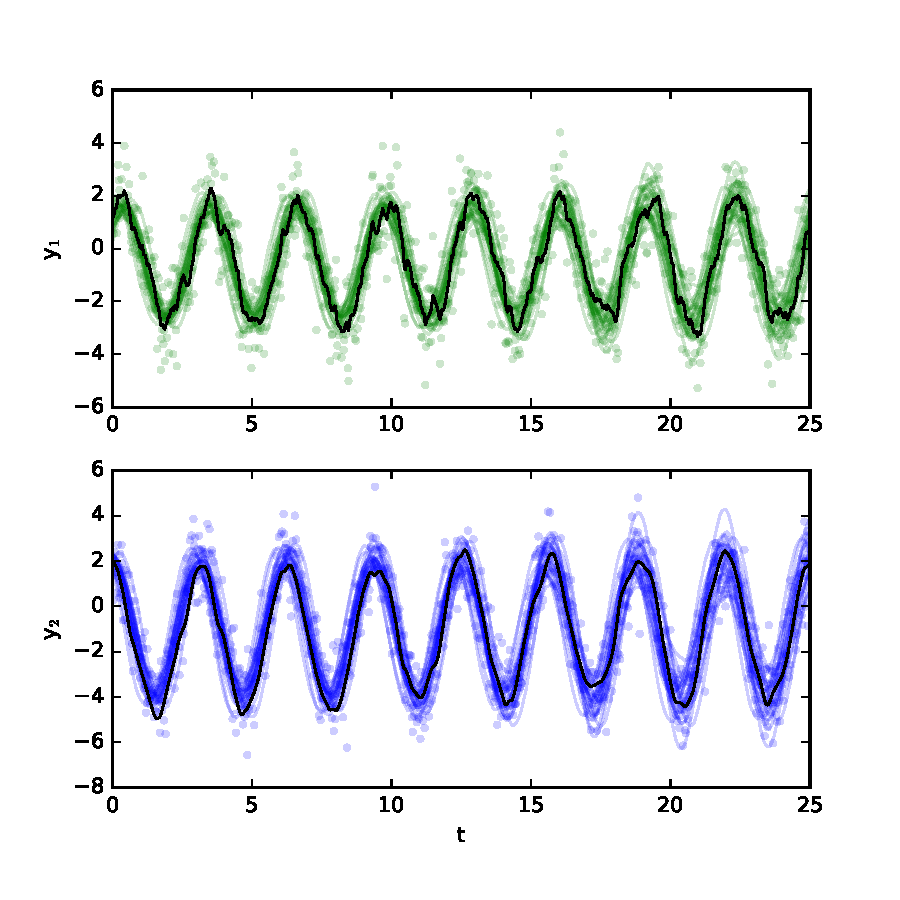
\includegraphics[width = 0.5\textwidth]{Figures/RTS_stoch_data}
\caption{The filtered data (black lines) compared with the noisy model (blue and green lines) and noisy data (blue and green dots).}
\label{fig:RTS_stoch_data}
\end{center}
\end{figure}


The particular variant of filter that I use (RTS smoother)   takes takes advantage of the fact that we have the entire time series in our possession and so ``know the future''. By integrating backwards the filter can better distinguish between signal and noise. We see that the filter identifies the noise remarkably well resulting in an output that is in fact extremely close to the analytical solution (Figure \ref{fig:RTS_analytical}).


\begin{figure}[htbp]
\begin{center}
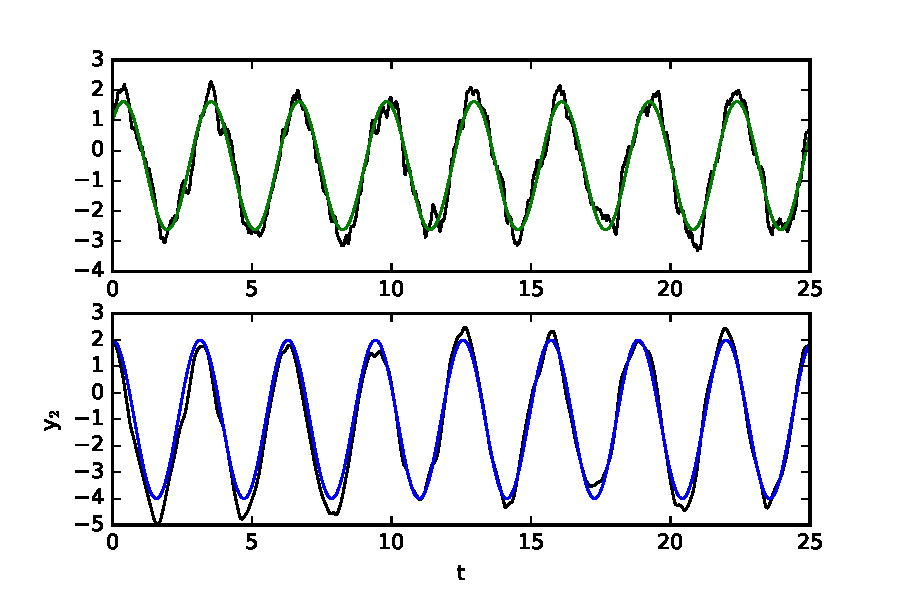
\includegraphics[width = 0.5\textwidth]{Figures/RTS_analytical}
\caption{The filtered data (black lines) plotted alongside the analytical solution.}
\label{fig:RTS_analytical}
\end{center}
\end{figure}


There are two more features of the Kalman filter that make it very handy. First, the states are not required to be directly observable. For instance, we may be able to see only a subset of the states, or some function of them (e.g.\ only position, rather than position and velocity). So for our model, here written in matrix form, we might have a measurement function $h = \begin{bmatrix}
1 & 0
\end{bmatrix}
$ that maps the states y to the observations z. 

\begin{align}
\begin{bmatrix}
\dot y_1 \\
\dot y_2
\end{bmatrix}
&= 
\begin{bmatrix}
-2 & 2 \\
-4 & 2
\end{bmatrix}
\,
\begin{bmatrix}
y_1 \\
y_2
\end{bmatrix}
+
\begin{bmatrix}
1 \\
0
\end{bmatrix}
\\
z &= 
\begin{bmatrix}
1 & 0
\end{bmatrix}
\begin{bmatrix}
y_1 \\
y_2
\end{bmatrix}
%
\end{align}

The second useful feature of the filter is that it allows for straightforward parameter estimation. Any parameters that are part of the system and whose values are imperfectly known can be designated as state variables, and so have the filter estimate their value alongside those of the actual states. For instance, in the above example, suppose the value of the forcing function was some unknown value $a$ rather than 1. Figure \ref{fig:RTS_Pest} shows how the filter converges onto the right value for the parameter, despite a far off initial guess. It also shows that we are provided an estimate for $y_2$ despite it being a latent state. 

\begin{align}
\begin{bmatrix}
\dot y_1 \\
\dot y_2 \\
\dot a
\end{bmatrix}
&= 
\begin{bmatrix}
-2 & 2 & 1 \\
-4 & 2 & 0 \\
0  & 0 & 0 
\end{bmatrix}
\,
\begin{bmatrix}
y_1 \\
y_2 \\
a
\end{bmatrix}
\\
z &= \begin{bmatrix}
1 & 0 & 0
\end{bmatrix}
\begin{bmatrix}
y_1 \\
y_2 \\
a
\end{bmatrix}
%
\end{align}



\begin{figure}[htbp]
\begin{center}
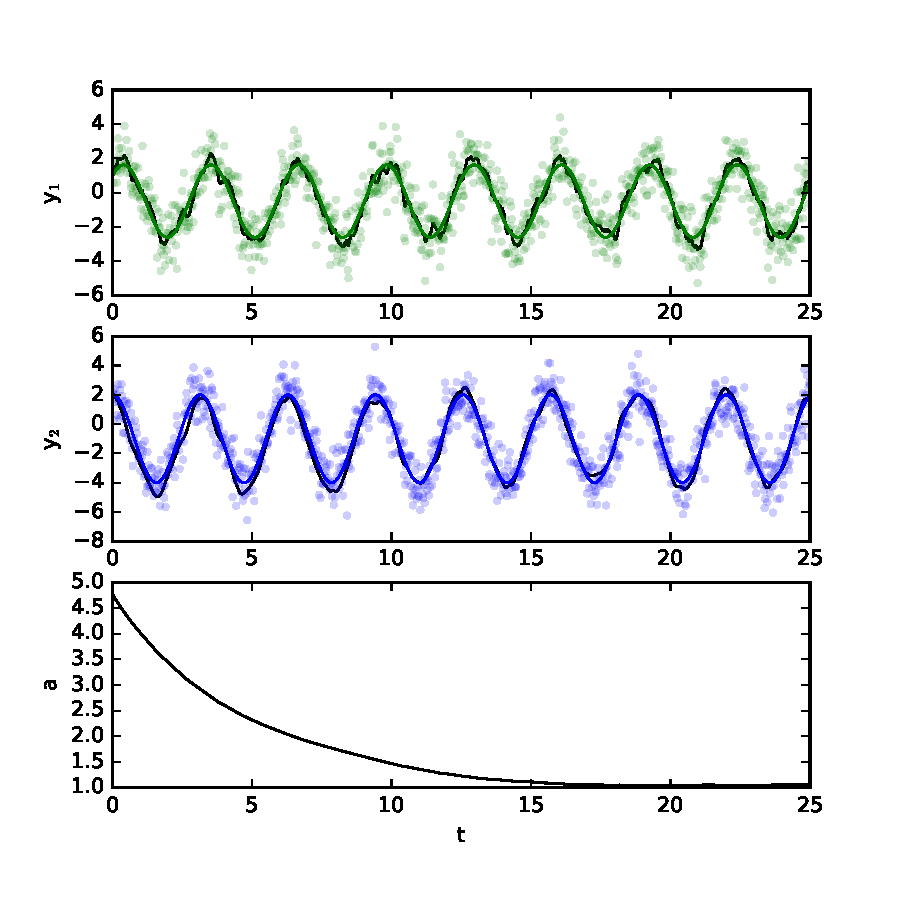
\includegraphics[width = 0.5\textwidth]{Figures/RTS_Pest}
\caption{The filtered data and estimated parameter (black lines) plotted alongside the noisy observations and analytical solution. %Notice how the value of the parameter converges to the correct value despite far-off initial guess. Also note that the filter provides an estimate for $y_2$ despite it being a latent (hidden) state.
}
\label{fig:RTS_Pest}
\end{center}
\end{figure}







\newpage{}


\section{Filtering of carbon cycle data}

%A simple model for mass variations in the ocean-atmosphere system is (Kump and Arthur, 1999):
%\begin{eqnarray}
%\frac{d M_p}{dt} &=& F_{wp} - F_{bp} \\ \nonumber
%\frac{d M_c}{dt} &=& F_{v} + F_{wo} - F_{ws} - F_{bo} 
%\end{eqnarray}
%
%These equations can be coupled to a model for ocean-atmosphere carbon isotope values. 
%%
%\begin{eqnarray}
%\frac{d\delta_c}{dt} = \frac{
%F_v\,(\delta_v - \delta_c) -
%F_{wo}\,(\delta_{wo} - \delta_c) +
%F_{bo}\,\epsilon  
%}{M_c}
%\end{eqnarray}
%
%In Figure \ref{fig:isotopes} the model is simulated with a 

%The model can be cast in linear form by a linear parameterization of the dependencies of the fluxes on the masses:
%\begin{eqnarray}
%\frac{d M_p}{dt} &=& k_{wp}\,M_{c} - k_{bp}\,M_p \\ \nonumber
%\frac{d M_c}{dt} &=& F_{v} + F_{wo} - k_{ws}\,M_c - k_{bo}\,M_p 
%\end{eqnarray}



\end{document}  







The important thing to note is while the isotope values depend on the mass balance, the mass balance does not depend on the isotopic mass balance. So rather than treating the ocean-atmosphere isotope values as a third state to be solved simultaneously with the other two, it is more appropriately thought of a a layer through which the states are propagated. This approach is commonly used in engineering practices, where a distinction is made between the equations that describe the states and the observations that are derived from them.
%\begin{eqnarray}
%\dot {\bf x} &=& f(\bf x) + {\bf \epsilon_{\bf x} }\\
%{\bf y} &=& g({\bf x}) + {\bf \epsilon_{\bf y} }\nonumber
%\end{eqnarray}
%
%Here ${\bf x}$ denotes a vector of states, ${\bf \dot x}$ their time derivatives, and $f({\bf x})$ a description of the time dependent behavior of the states. The integrated values of the states are then propagated through another layer $g({\bf x})$ which maps the states to observations ${\bf y}$. 
%
One advantage of this approach is that often some or all of the states are unobservable (latent), while one of more of the observables can be tracked directly with sensors or measurements. For instance, one may be able to track the position of a vehicle with GPS, but not have direct measurements of velocity and acceleration, which are part of the equations of motion of the vehicle. 
%
A second advantage is that the recognition of two distinct layers, the state equations, and the observation equations, allow ascribing each layer with its own source of noise. The model describing the behavior of the states might have uncertainties associated with some of its parameters, and so might the observations have some measurement noise associated with them. 
 
%If the relationships described by $g$ and $f$ are linear, then they can be described using matrices:
%\begin{eqnarray}
%\dot {\bf x} &=& A{\bf x} + B{\bf u}\\
%{\bf y} &=& C{\bf x} + D{\bf u}\nonumber
%\end{eqnarray}
%
%Here $A$ is the dynamics or state matrix, $B$ is the input matrix, $C$ is the output matrix, and $D$ is the feed-forward matrix. $u$ is a vector of inputs/forcings that are external to the system being modeled. If the matrices are constant with time then this form is known as the state-space representation of a linear time-invariant (LTI) system. 

For the carbon cycle, if the dependencies of the fluxes on the reservoirs are assumed to be of first-order and constant through time (or at least slowly-varying relative to the duration of interest), then a linear form can be written:

\begin{equation}\label{eq:matform}
 \left[ 
\begin{matrix}
\dot M_p \\
\dot M_c
\end{matrix}
\right]  
=
\left[
\begin{matrix}
-k_{bp}	   & k_{wp}  \\
-k_{bo} 	& -k_{ws} 
\end{matrix}
\right]
\left[
\begin{matrix}
M_p \\
M_c
\end{matrix}
\right] 
+
\left[
\begin{matrix}
0 \\
F_{v} + F_{wo}
\end{matrix}
\right] 
\end{equation}
%
Or with the notation used in Bachan et al. (201x) using arrows to indicate vectors and underline to indicate matrices:
%
\begin{equation}\label{eq:linsys_matform}
\dot{\vec{M}} = \underline K {\vec{M}} + \vec{F}
\end{equation}

Thus, the mass balance equations can be written in linear form without great compromise of the accuracy of the physical representation. The isotopic mass balance, however, is inherently non-linear since it involves products of isotopic composition and mass which gives rise to $M_c$ in the denominator. 
\begin{eqnarray}
\dot{\vec{M}} &=& \underline K {\vec{M}} + \vec{F} + {\bf \epsilon_{\bf x} }\\
\dot \delta_c &=& g(\vec M, \vec F) + {\bf \epsilon_{\bf \delta} }\nonumber
\end{eqnarray} 
 
This recasting of the equations of mass balance and isotopic mass balance in state-space form is useful as it allows accurately representing the reality that while the measurement layer is visible to us through measurements of carbon isotopic values in marine carbonates, the states (mass of carbon and phosphate in the ocean) remain hidden from us in deep time.  It also allows ascribing each layer its own sources of noise. The latter is particularly important as the sources of variance propagate very differently through the system of equations and have different impacts on the resulting isotopic signal. 




\section{Kalman Filter}

Given some knowledge of the structure of the variance in the state estimates, and error in the observations, it is natural to ask whether an estimate can be obtained that simultaneously minimizes both sources of error. Such an estimate is given by the Kalman Filter. Moreover, for a wide class of systems with Gaussian noise and a linear state equations, the filter can be shown to provide the best possible estimate, that is, the state estimates that are  closest to the true states. 

The filter is often cast in a form that consists of two steps: prediction and update. The predict step:
\begin{eqnarray}
x_t &=& F x_{t-1} + B u \\
P_t &=& F P_{t-1} F^T + Q \nonumber
\end{eqnarray}


The update step generates estimates for the state and covariance:

\begin{eqnarray}
\hat x_t &=& x_t + K(z_t - H x_t) \\
\hat P &=& (I - K H) P \\
K &=& P H^T (HPH^T + R)^{-1}
\end{eqnarray}

For application of the filter let us use the synthetic data we produced earlier. 


\section{Ensemble Kalman Filter}



\newpage{}


\appendix

\section{Discretization of Carbon Cycle Equations}

The discrete versions of the mass balance and isotopic mass balance equations are:
%\begin{eqnarray}
%\frac{\Delta M_p}{\Delta t} &=& k_{wp}\,M_{c} - k_{bp}\,M_p \\ \nonumber
%\frac{\Delta M_c}{\Delta t} &=& F_{v} + F_{wo} - k_{ws}\,M_c - k_{bo}\,M_p 
%\end{eqnarray}
%
%\begin{eqnarray}
%\frac{\Delta M_p(t) - M_p(t-1)}{\Delta t} &=& k_{wp}\,M_{c} - k_{bp}\,M_p \\ \nonumber
%\frac{\Delta M_c(t) - M_c(t-1)}{\Delta t} &=& F_{v} + F_{wo} - k_{ws}\,M_c - k_{bo}\,M_p 
%\end{eqnarray}
%
\begin{eqnarray}
{ M_p^k} &=& M_p^{k-1} + {\Delta t}\Big(k_{wp}\,M_{c}^{k-1} - k_{bp}\,M_p^{k-1}\Big) \nonumber \\[0.5em] 
%
{ M_c^k} &=& M_c^{k-1} + {\Delta t}\Big( F_{v} + F_{wo} - k_{ws}\,M_c^{k-1} - k_{bo}\,M_p^{k-1} \Big) \nonumber \\[0.5em] 
%
{\delta_c^k} &=& \delta_c^{k-1} + {\Delta t}\frac{
F_v\,\big(\delta_v - \delta_c^{k-1}\big) -
F_{wo}\,\big(\delta_{wo} - \delta_c^{k-1}\big) -
k_{bo}\,M_p^{k-1}  
}{M_c^k} \nonumber
%
\end{eqnarray}

Rearranging:

\begin{eqnarray}
{ M_p^k} &=& \Big(1 - {\Delta t}k_{bp}\Big)M_p^{k-1} + {\Delta t}k_{wp}\,M_{c}^{k-1}\nonumber \\[0.5em] 
%
{ M_c^k} &=& \Big(1 - {\Delta t}k_{ws} \Big)M_c^{k-1}   - {\Delta t}k_{bo}\,M_p^{k-1} + {\Delta t} F_{v} +{\Delta t} F_{wo}\nonumber 
\\[0.5em] 
%
{\delta_c^k} &=& \Big( 1 - 
\frac{ {\Delta t}F_v }{M_c^{k-1}} + 
\frac{ {\Delta t}F_{wo}}{M_c^{k-1}} \Big)\delta_c^{k-1} -
\frac{ {\Delta t}k_{bo}\,M_p^{k-1} }{M_c^{k-1}} +
\frac{ {\Delta t}F_v\,\delta_v}{M_c^{k-1}} -
\frac{ {\Delta t}F_{wo}\,\delta_{wo}}{M_c^{k-1}}
\nonumber
%
\end{eqnarray}








%
%\begin{equation}\label{eq:matform}
% \left[ 
%\begin{matrix}
%M_p^{k+1} \\
%M_c^{k+1}
%\end{matrix}
%\right]  
%=
%\left[
%\begin{matrix}
%1 - \Delta t \, k_{bp}	   & \Delta t \, k_{wp}  \\
%- \Delta t \, k_{bo} 	& 1 - \Delta t \, k_{ws} 
%\end{matrix}
%\right]
%\left[
%\begin{matrix}
%M_p^k \\
%M_c^k
%\end{matrix}
%\right] 
%+
%\left[
%\begin{matrix}
%0 \\
%\Delta t \, (F_{v} + F_{wo})
%\end{matrix}
%\right] 
%\end{equation}
%%

















